\documentclass[tikz,border=2pt]{standalone}
\usepackage{tikz}
\usepackage[european]{circuitikz}
\usetikzlibrary{arrows.meta,positioning,calc}
../cictikz/src/cictikz/data/tex/cictikz_lib.tex
\begin{document}
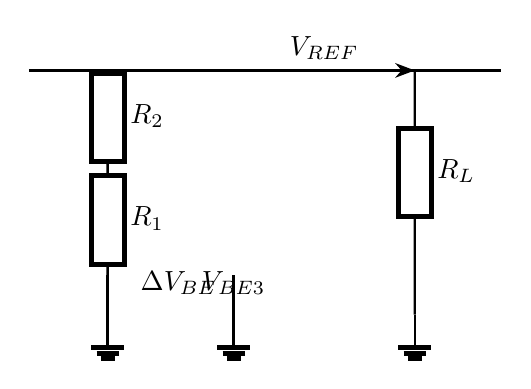
\begin{tikzpicture}[>=Stealth, line width=0.9pt]
  \draw (0,3.0) -- (6,3.0);
  \draw (1.0,3.0) to[resistor,l=$R_2$] (1.0,1.8);
  \draw (1.0,1.8) to[resistor,l=$R_1$] (1.0,0.4);
  \draw (1.0,0.4) -- (1.0,-0.1) node[ground] {};
  \node at (1.9,0.3) {$\Delta V_{BE}$};
  \draw (2.6,0.4) -- (2.6,-0.1) node[ground] {};
  \node at (2.6,0.3) {$V_{BE3}$};
  \draw[->] (2.6,3.0) -- (4.9,3.0) node[midway,above] {$V_{REF}$};
  \draw (4.9,3.0) to[resistor,l=$R_L$] (4.9,0.4) -- (4.9,-0.1) node[ground] {};
\end{tikzpicture}
\end{document}
